%!TEX root = ../dissertation.tex
\begin{savequote}[75mm]
This is some random quote to start off the chapter.
\qauthor{Firstname lastname}
\end{savequote}

\chapter{Model and approach}

\todo{rivedere il titolo del capitolo}

SCALETTA:

* Visual branch
  * proposal 
  * object generator
* textual branch
  word embedding (w2v, glove)
* concept branch
* loss
* training and inference

\section{Model}

In the following sections we describe the model architecture, outlined
in Fig.\ref{fig:model-architecture}.

\begin{figure}
  \centering
  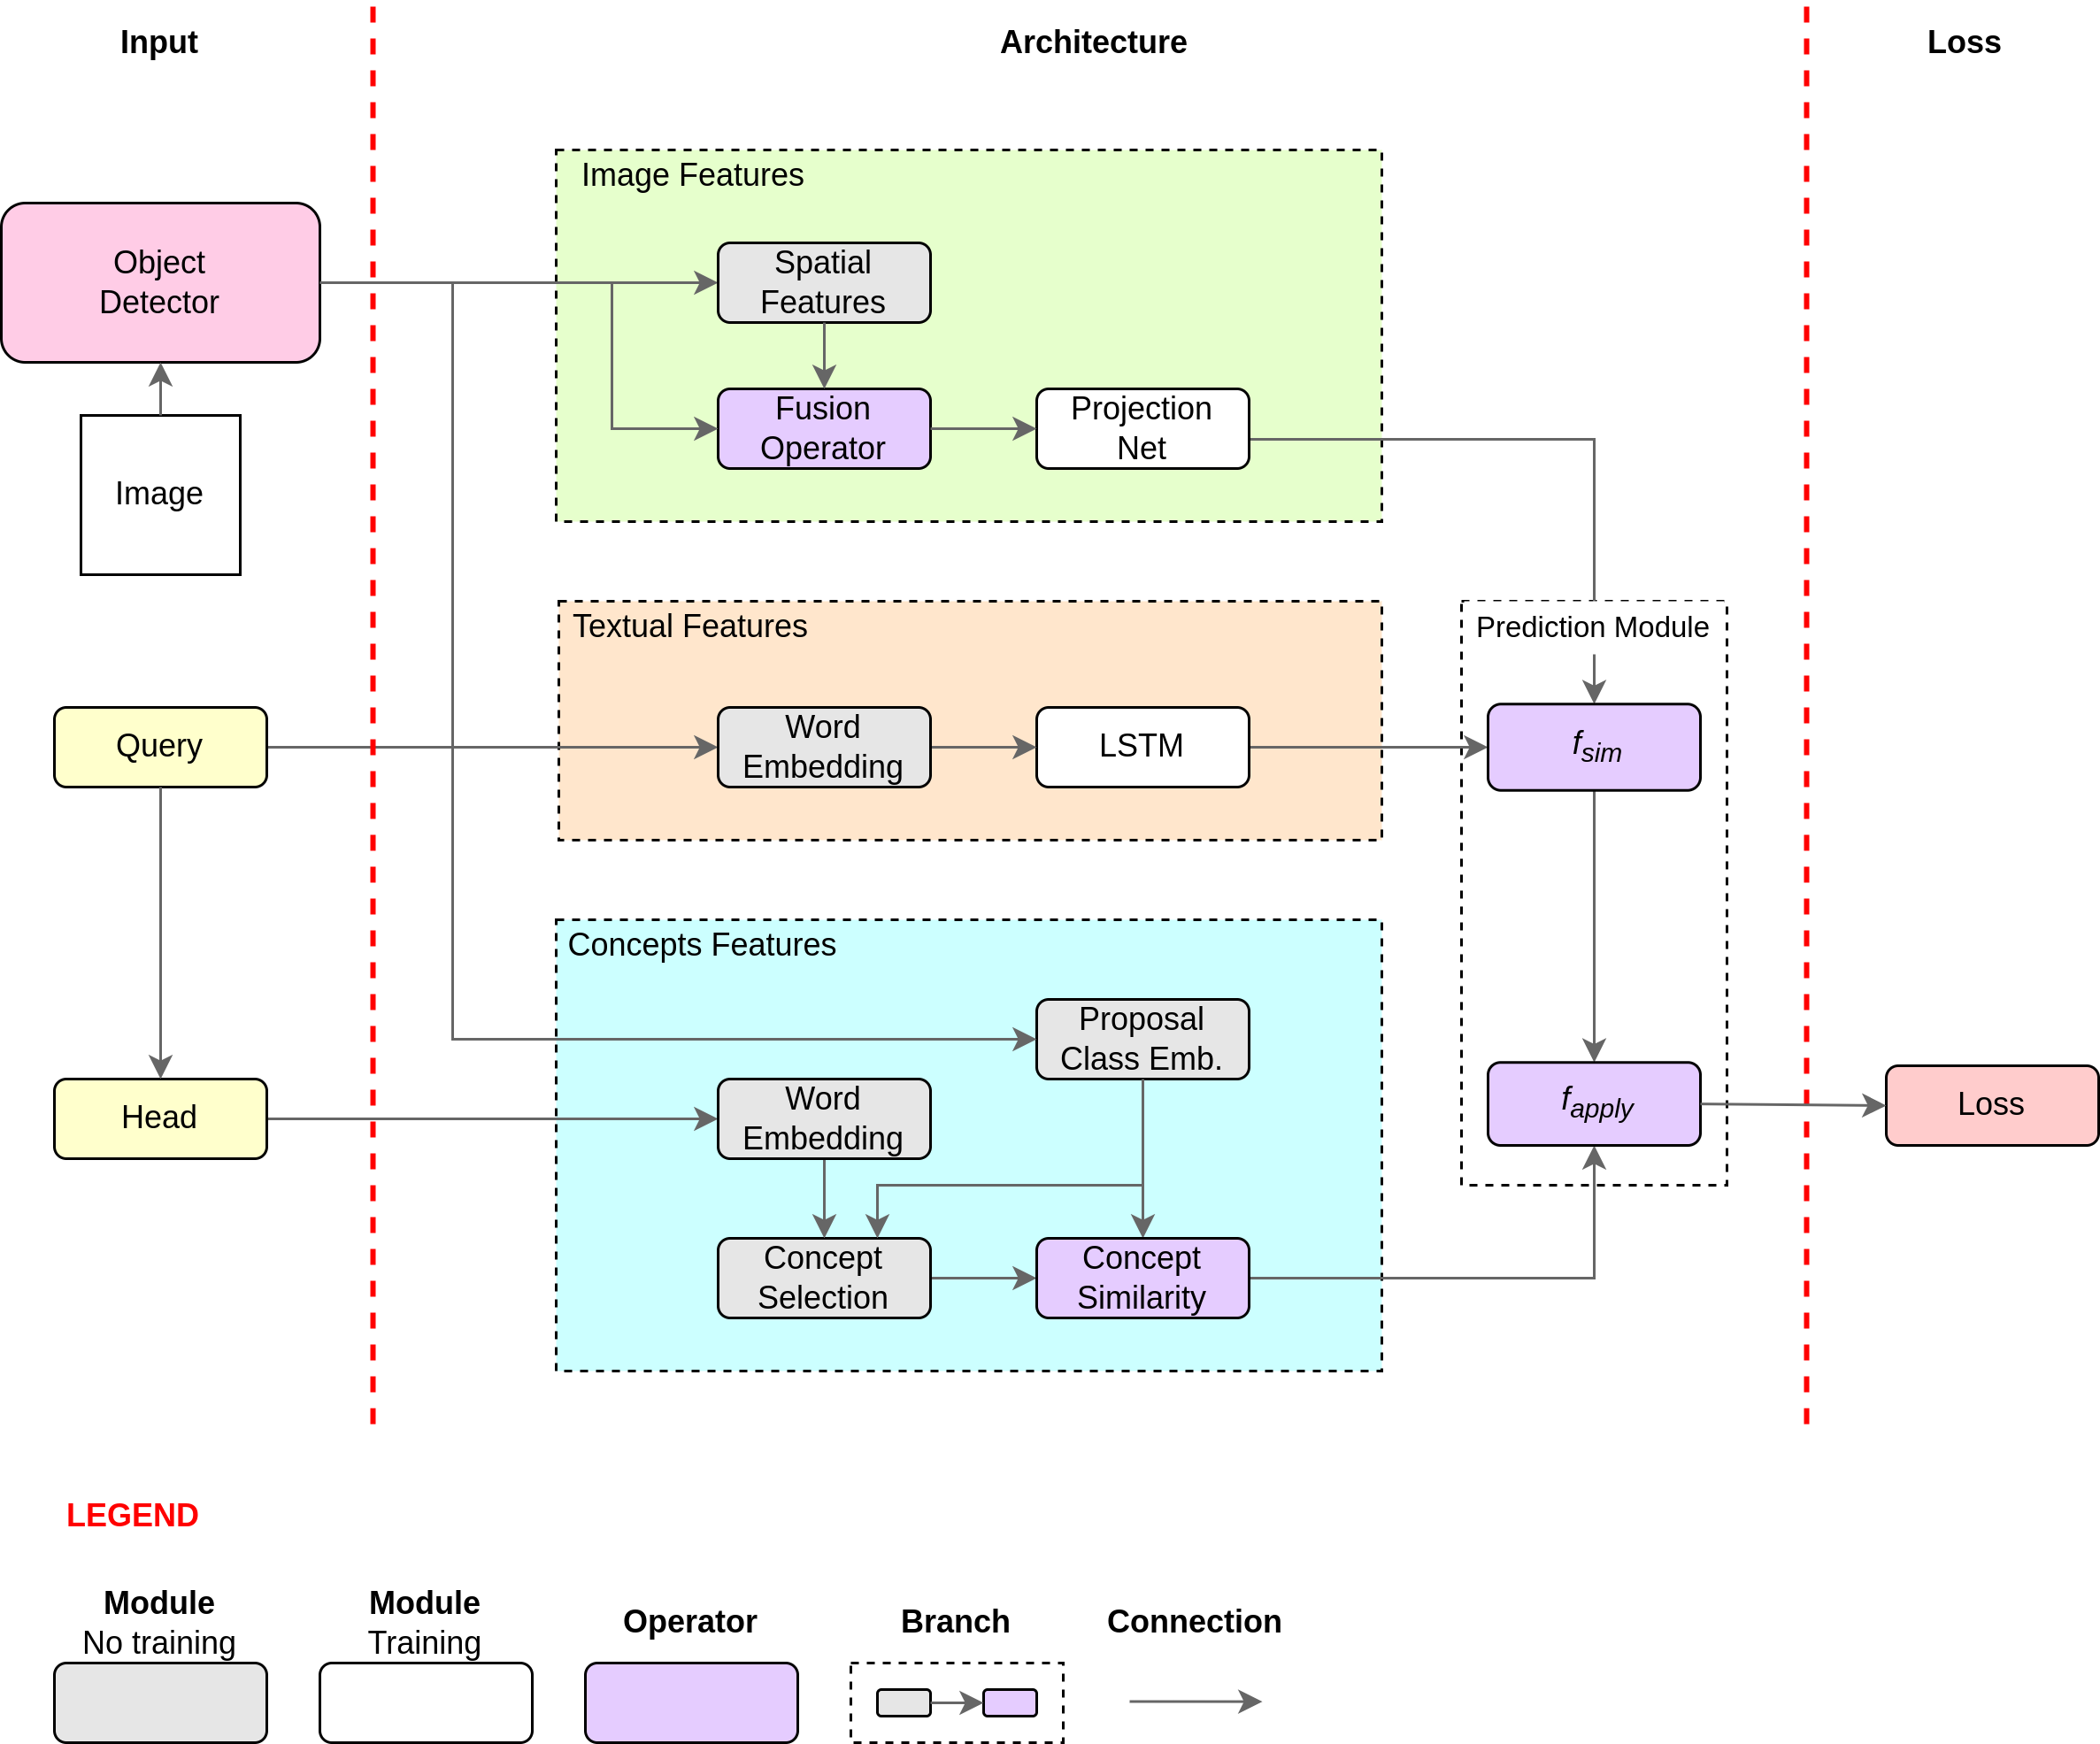
\includegraphics[width=1.0\textwidth]{figures/model-architecture.png}
  \caption[TODO]{Our model architecture overview. [WORK IN PROGRESS]}
  \label{fig:model-architecture}
\end{figure}

Our model, outlined in Fig.~\ref{fig:model-architecture}, follows a
typical basic architecture for visual textual grounding tasks. It is
based on a two-stage approach in which, initially, a pre-trained
object detector (see Sec.~\ref{sec:object-detection-recognition}) is
used to extract, from a given image $\bm{I}$, a set of $k$ bounding
box proposals $\calP_{\bm{I}} = \{ \bm{p}_i \}^k_{i=1}$, where $p_i
\in \Rset^4$, jointly with features $H^v = \{ \bm{h}^v_i \}^k_{i=1}$,
where $\bm{h}^v_i \in \Rset^v$. The features represent the internal
object detector activation values before the classification layers and
regression layer for bounding boxes. Moreover, our model extracts the
spatial features $H^s = \{ \bm{h}^s_i \}^k_{i=1}$, where $\bm{h}^s_i
\in \Rset^s$ from all the bounding boxes proposals, with the spatial
features for the proposal $\bm{p}_i$ defined as:
\begin{equation}
  \bm{h}^s_i = \left[ \frac{x1}{wt}, \frac{y1}{ht}, \frac{x2}{wt}, \frac{y2}{ht}, \frac{(x2 - x1) \times (y2 - y1)}{wt \times ht}  \right]
\end{equation}
where $(x1, y1)$ refers to the top-left bounding box corner, $(x2,
y2)$ refers to the bottom-right bounding box corner, $wt$ and $ht$ are
the width and height of the image, respectively. Both visual and
spatial features are then concatenated, thus leading to a set of new
vectorial representations $H^{||} = \{ \bm{h}^{||}_{jz} \}_{j \in [1,
\ldots, m], z \in [1, \ldots, k]}$, where vectors $\bm{h}^{||}_{jz}$
are defined as:
\begin{equation}
  \bm{h}^{||}_{jz} = \Big( \bm{W}^{||} \left( \bm{h}^s_z || L1(\bm{h}^v_z) \right) + \bm{b}^{||} \Big) 
\end{equation}
where $||$ indicates the concatenation operator, $\bm{h}^{||}_{jz} \in
\Rset^c$, $\bm{W}^{||} \in \Rset^{c \times (s + v)}$ is a matrix
of weights, and $\bm{b}^{||} \in \Rset^c$ is a bias vector.

We also assume that the object detector returns, for each $\bm{p}_i$,
a probability distribution $Pr_{Cls}(\bm{p}_i)$ over a set $Cls$ of
predefined classes, i.e. the probability for each class $\zeta \in
Cls$ that the content of the bounding box $\bm{p}_i$ belongs to
$\zeta$. This information is typically returned by most of the object
detectors, and it will be used to define our novel loss function.
\todo{UPDATE: to define our...}

\subsection{Textual Branch}

Regarding the textual features extraction, given a noun phrase
$\bm{q}_j$, initially all its words $W^{\bm{q}_j} = \{ w^{\bm{q}_j}_i
\}^l_{i=1}$ are embedded in a set of vectors $E^{\bm{q}_j} =
\{e^{\bm{q}_j}_i \}^l_{i=1}$ where $e^{\bm{q}_j}_i \in \Rset^w$, where
$w$ is the size of the embedding. Then, our model applies a LSTM (see
Sec.~\ref{subsec:gated-rnn}) neural network to generate from the
sequence of word embeddings only one new embedding $\bm{h}^*_j$ for
each phrase $\bm{q}_j$. This textual features extraction is defined
as:
\begin{equation}
  \bm{h}^*_j = L1(LSTM(E^{\bm{q}_j}))
\end{equation}
where $\bm{h}^*_j \in \Rset^t$ is the LSTM output of the last word in
the noun phrase $\bm{q}_j$ , and $L1$ is the L$1$ normalization
function.

\subsection{Similarity Branch}

Along with visual and textual features we also compute a similarity
score beween noun phrases and bounding box class labels. Such score is
crucial for learning to ground, and we call it concept similarity. The
idea behind this is straightforward: the more the noun phrase and the
councept expressed throught the bounding box label are semantically
similar, the more they are related. In a weakly-supervised scenario
where we are missing the grounding information, to known whether a
phrase and the concept that it expresses (i.e, the bounding box) are
related is very important for the learning process. Here, an
assumption is made: the bounding box class label semantically define
the content of the bounding box. 

Formally, given set of proposal $\calP^{\bm{I}}$ and a noun phrase
$\bm{q}_j$, we compute the concept similarity score for each proposal
$i$ and phrase $j$ as:
\begin{equation}
  \bm{S}^c_{ji} = \fsim \left( \xi, \ePI_i \right),
\end{equation}
where $\fsim$ is a similarity measure such us the cosine similarity,
$\ePI_i$ is the embedding of the class for the $i$-th proposal, and
$\xi$ is the embedding representing the concept of the noun phrase
$\qj$:
\begin{equation}
  \xi = \fagg(\Eqj, \EPI).
\end{equation}
Please note that we use the same notation for proposal class
embeddings: $\EPI = \{ \ePI_i \}^{k}_{i=1}$ is the set of embeddings,
one per proposal, representing the bounding box class label. Moreover,
for each proposal we consider only the embedding of the class with
maximum probability: $\max Pr_{Cls} (\bm{p}_i)$, i.e., every proposal
is associated with one class label. \todo{ADD: problema del background
delle calssi} The new embedding $\xi$ can be computed with different
strategies: for example, we can simply compute the mean of all word
embeddings in the noun phrase:
\begin{equation}
  \fagg^{\text{mean}}(\Eqj, \EPI) = \frac{\sum^l_{i=1} \eqj_i}{| \Eqj |},
\end{equation}
or use only the last word as done in \todo{CITE: Phrase Loc
wo Paired Training Examples}:
\begin{equation}
  \fagg^{\text{last}}(\Eqj, \EPI) = \eqj_l.
\end{equation}
More complex strategies instead take into account external
information, such us the similarity wrt proposal class embeddings.
Here, we compute the similarity between word in noun phrase and
proposal class embeddings and then we select one word in the noun
phrase with maximum similarity wrt the detected concept in proposal:
\begin{equation}
  \fagg^{\text{max}}(\Eqj, \EPI) = \max_{\eqj \in \Eqj} \{ \max g(\eqj) \},
\end{equation}
where
\begin{equation}
  g(\eqj) = \{ \fsim(\ePI, \eqj) \mid \ePI \in \EPI \}.
\end{equation}

\subsection{Prediction Module}

Finally, the model predicts the probability $\bm{P}_{jz}$ that a given
noun phrase $\qj$ is referrred to a proposal bounding box $\bm{p}_z$
as:
\begin{equation}
  \bm{P}_{jz} = \fsim ( \bm{h}^{||}_{jz} , \bm{h}^*_j ).
\end{equation}
Here, $c$ should be equal to $t$, where $c$ and $t$ are the dimension of vector,
respectively $\bm{h}^{||}_{jz} \in \Rset^c$ and $\bm{h}^*_j \in
\Rset^t$.

As noted in \todo{CITE: kak net}, concept similarit is a direct
consequence of the intrinsic knwoledge convoyed by the object
detector. This can be exploited to instruct the model on what to
focus. The idea behind this is simple but effective: given the concept
similarity, that is, the similarity of concept expressed in phrase wrt
the content of the bounding box, we can use it as a prior for the
model and down-weight unrelated proposals. Hence, we can apply the
concept similarity on previously computed $\bm{P}_{jz}$ as:
\begin{equation}
  \bm{P}^*_{jz} = \fapplysim \left( \bm{P}_{jz} , \bm{S}^c_{jz} \right).
\end{equation}

For the sake of presentation, we show that $\bm{P}_{jz}$ is equal to
$\bm{P}^*_{jz}$ by applying concept similarity on $\bm{P}$ with
$\fapplysim^{\text{one}}$, a funcion that simply ignore $\bm{S}^c$
matrix:
\begin{equation}
  \fapplysim^{\text{one}} (\bm{S}^c_{jz}, \bm{P}_{jz}) = \bm{P}_{jz}.
\end{equation}
Outside of this section, we use the notation $\bm{P}^*$ for referring
to the predictions matrix, and whether the concept similarity is
applied or not is an implementation detail.

The simplest strategy for applying the concept similarity to
previously computed predictions is by multiplying the two, treating
$\bm{S}^c_{jz}$ as a weight matrix:
\begin{equation}
  \fapplysim^{\text{prod}} (\bm{S}^c_{jz}, \bm{P}_{jz}) = \bm{S}^c_{jz} * \bm{P}_{jz}.
\end{equation}

At first glance, this approach seems very promising because we force
the model to return predictions ``on steroid'' when there is a
semantic relation between phrase and proposal or downweighted when no
similarity is found. However, this relies on the assumption that the
embedding space and similarity measure we are using for words
perfectly captures the semantic similarity between them, and this is
not true. Also, we assume that proposals are classified with no error
by the object detector, neither this is true. Under those hypotesis,
such application of concept similarity cannot be fruitful. 

An example my clarify our statement. We are given $\bm{S}^c \in
\Rset^{1 \times 2}$, $\bm{S}^c = [0.1, 0.2]$ for an example composed by a
phrase and two proposal, and we know that the bounding box to ground
with our prhrase is the first. The only way the model has to output
the first proposal as the best bounding box, i.e., the bounding box to
ground, is to predict a score $p_{0}$ which is at least the double of
$p_{1}$, because
\begin{equation}
  \bm{P}^* = [0.1 * p_{0}, 0.2 * p_{1}]
\end{equation}
where $p_{j} = \bm{P}[0, j]$, and 
\begin{equation}
\begin{split}
0.1 * p_{0} > 0.2 * p_{1} & \iff p_{0} >  \frac{0.2}{0.1} * p_{1} \\
  & \iff p_{0} > 2 * p_{1}.
\end{split}
\end{equation}
Thus, with such scores $\bm{S}^c$, when the model predicts $0.1$ for
$p_1$, it must learn to predict $> 0.2$ for $p_0$, when it predicts
$0.5$ for $p_1$, it must learn to predict $1.0$ for $p_0$ and when it
predicts a value $> 0.5$ for $p_1$ there is no way to predict a
greater score for $p_0$. In conclusion, it's very difficult to learn
to ground in such settings and given problems highlighted above.

A more convenient way of applying concept similarity to prediction is
instead to compute the mean between two. Eventually, we can also put a
weight on two terms in order to balance contributions. Formally,
$\fapplysim$ becomes:
\begin{equation}
  \fapplysim^{\text{mean}} (\bm{S}^c_{jz}, \bm{P}_{jz}) = (1 - \lambda) * \bm{S}^c_{jz} + \lambda * \bm{P}_{jz}.
\end{equation}

\section{Training}

In this section, we present our loss. For the sake of presentation, we
define in the following the loss terms referred to a single example.
The total loss is then obtained by summing up the contributions of all
examples in the training set.

Please note that in weakly-supervised settings, for a training example
$\left( \bm{I}, S \right)$ we are not given the query-proposal pair
set $\{ ( q^{gt}_j, p^{gt}_j ) \}^m_{j=1}$, where $m$ is the number of
noun phrases.
% Thus, how can instruct our model to learn without the ground truth?
% This problem is well known in literature: in \todo{CITE: align2ground}
% they enforces the score between a noun phrase and a proposal to be
% higher than a non-paired proposal, and vice-versa. In ...
To tackle this problem, in our work we adopt a very simple strategy:
we exploit concept similarity. Basically, we consider ``positive'' an
example where the concept similarity is above a certain treshold, and
``negative'' an example whose concept similarity is below threshold:
\begin{equation}
  \bm{D}_{jz} =
  \begin{cases}
    0, & \bm{S}^c_{jz} > \sigma \\
    1, & \text{otherwise}
  \end{cases},
\end{equation}
 \todo{FIX: equation: out are in -1, 0, 1}
where $\bm{S}^c$ is the concept similarity. This policy relies on the
assumption that concept similarity correctly captures the semantic
relation between query and proposal. $\bm{D}$ is the concept direction
matrix.

Now, given a training example $\left( \bm{I}, S \right)$, where
$\cal{P}_{\bm{I}}$ the bounding box proposals set, we define the loss
function $\calL$ (for a single example) as:
\begin{equation}
  \calL = \frac{1}{m} \sum^m_{j=1} \Bigg( \frac{1}{z} \sum^k_{z=1} \floss ( \bm{P}^*_{jz}, \bm{D}_{jz} ) \Bigg)
\end{equation}
where $m$ in the number of noun phrases, $k$ is the number of proposal
bounding box, $\bm{P}^*_{jz}$ is the model predicted probability that
the noun phrase $\bm{q}_j \in \calQ$ refers to the image content
localized by $\bm{p}_z \in \calP_{\bm{I}}$. Our loss is scaled by $m$
and $k$ because number of noun phrase can change, but also number of
proposal: in our case, we ignore proposal with class label equal to
``background'' (see Sec.~\todo{REF: sec}). In the end, $\floss$ is the
function that optimize the learning process by combining predicted
scores with the concept direction. TODO: many strategie can apply, but
we chose...\todo{TODO: complete sentence}
\begin{equation}
  \floss ( \bm{P}^*_{jz}, \bm{D}_{jz} ) = -1 * ... % TODO \bm{D}_{jz} * x_pos + torch.square(y * x_neg)
\end{equation}
\todo{FIX: equation}
